\usetikzlibrary{calc}
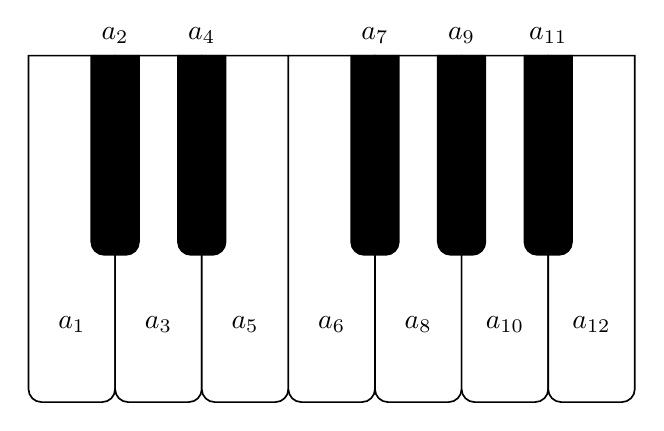
\begin{tikzpicture}[x=1.1cm,y=1.1cm,line width=.6pt]
% --- white keys (7): each [k,k+1]x[0,4], bottom corners r=0.15 ---
\draw[fill=white] (0,4.0) -- (0,0.15) arc(180:270:0.15) -- (0.85,0) arc(270:360:0.15) -- (1,0.15) -- (1,4.0) -- cycle; %WK0
\draw[fill=white] (1,4.0) -- (1,0.15) arc(180:270:0.15) -- (1.85,0) arc(270:360:0.15) -- (2,0.15) -- (2,4.0) -- cycle; %WK1
\draw[fill=white] (2,4.0) -- (2,0.15) arc(180:270:0.15) -- (2.85,0) arc(270:360:0.15) -- (3,0.15) -- (3,4.0) -- cycle; %WK2
\draw[fill=white] (3,4.0) -- (3,0.15) arc(180:270:0.15) -- (3.85,0) arc(270:360:0.15) -- (4,0.15) -- (4,4.0) -- cycle; %WK3
\draw[fill=white] (4,4.0) -- (4,0.15) arc(180:270:0.15) -- (4.85,0) arc(270:360:0.15) -- (5,0.15) -- (5,4.0) -- cycle; %WK4
\draw[fill=white] (5,4.0) -- (5,0.15) arc(180:270:0.15) -- (5.85,0) arc(270:360:0.15) -- (6,0.15) -- (6,4.0) -- cycle; %WK5
\draw[fill=white] (6,4.0) -- (6,0.15) arc(180:270:0.15) -- (6.85,0) arc(270:360:0.15) -- (7,0.15) -- (7,4.0) -- cycle; %WK6
% --- full-height divider at x=3 (no black key) reinforced ---
\draw (3,4.0) -- (3,0.15);
% --- black keys (5): width 0.55, y in [1.7,4.0], bottom r=0.15 ---
\fill[black] (0.725,4.0) -- (0.725,1.85) arc(180:270:0.15) -- (1.125,1.70) -- (1.125,1.70) arc(270:360:0.15) -- (1.275,1.85) -- (1.275,4.0) -- cycle; %BK1
\draw[black] (0.725,4.0) -- (0.725,1.85) arc(180:270:0.15) -- (1.125,1.70) arc(270:360:0.15) -- (1.275,1.85) -- (1.275,4.0) -- cycle;
\fill[black] (1.725,4.0) -- (1.725,1.85) arc(180:270:0.15) -- (2.125,1.70) -- (2.125,1.70) arc(270:360:0.15) -- (2.275,1.85) -- (2.275,4.0) -- cycle; %BK2
\draw[black] (1.725,4.0) -- (1.725,1.85) arc(180:270:0.15) -- (2.125,1.70) arc(270:360:0.15) -- (2.275,1.85) -- (2.275,4.0) -- cycle;
\fill[black] (3.725,4.0) -- (3.725,1.85) arc(180:270:0.15) -- (4.125,1.70) -- (4.125,1.70) arc(270:360:0.15) -- (4.275,1.85) -- (4.275,4.0) -- cycle; %BK3
\draw[black] (3.725,4.0) -- (3.725,1.85) arc(180:270:0.15) -- (4.125,1.70) arc(270:360:0.15) -- (4.275,1.85) -- (4.275,4.0) -- cycle;
\fill[black] (4.725,4.0) -- (4.725,1.85) arc(180:270:0.15) -- (5.125,1.70) -- (5.125,1.70) arc(270:360:0.15) -- (5.275,1.85) -- (5.275,4.0) -- cycle; %BK4
\draw[black] (4.725,4.0) -- (4.725,1.85) arc(180:270:0.15) -- (5.125,1.70) arc(270:360:0.15) -- (5.275,1.85) -- (5.275,4.0) -- cycle;
\fill[black] (5.725,4.0) -- (5.725,1.85) arc(180:270:0.15) -- (6.125,1.70) -- (6.125,1.70) arc(270:360:0.15) -- (6.275,1.85) -- (6.275,4.0) -- cycle; %BK5
\draw[black] (5.725,4.0) -- (5.725,1.85) arc(180:270:0.15) -- (6.125,1.70) arc(270:360:0.15) -- (6.275,1.85) -- (6.275,4.0) -- cycle;
% --- labels: white inside, black above (gap, never on lines) ---
\node[inner sep=0pt,anchor=center] at (0.5,0.9) {$a_{1}$};
\node[inner sep=0pt,anchor=center] at (1.5,0.9) {$a_{3}$};
\node[inner sep=0pt,anchor=center] at (2.5,0.9) {$a_{5}$};
\node[inner sep=0pt,anchor=center] at (3.5,0.9) {$a_{6}$};
\node[inner sep=0pt,anchor=center] at (4.5,0.9) {$a_{8}$};
\node[inner sep=0pt,anchor=center] at (5.5,0.9) {$a_{10}$};
\node[inner sep=0pt,anchor=center] at (6.5,0.9) {$a_{12}$};
\node[inner sep=0pt,anchor=south,yshift=4pt] at (1.0,4.0) {$a_{2}$};
\node[inner sep=0pt,anchor=south,yshift=4pt] at (2.0,4.0) {$a_{4}$};
\node[inner sep=0pt,anchor=south,yshift=4pt] at (4.0,4.0) {$a_{7}$};
\node[inner sep=0pt,anchor=south,yshift=4pt] at (5.0,4.0) {$a_{9}$};
\node[inner sep=0pt,anchor=south,yshift=4pt] at (6.0,4.0) {$a_{11}$};
\end{tikzpicture}
